\documentclass{beamer}
\usetheme{default}
\addtobeamertemplate{navigation symbols}{}{%
    \usebeamerfont{footline}%
    \usebeamercolor[fg]{footline}%
    \hspace{1em}%
    \insertframenumber/\inserttotalframenumber
}

\usepackage[utf8]{inputenc}
\usepackage{graphicx}
\usepackage{subfig}
\captionsetup[figure]{labelformat=empty}

\titlegraphic{
    
\includegraphics[width=4cm]{LOGO_PTYS_2017_Paysage.png}%
}

\title{Virtualisation des infrastructures}
\author{Productys}
\date{20 Janvier 2021}

\begin{document}

%====================================
%================1===================

\frame{\titlepage}


%====================================
%================3===================

\begin{frame}
\frametitle{Introduction}
Evolution des architectures systèmes et réseaux vers des solutions distribuées
\medbreak
Gestion simplifiée et sécurisée des infrastructures (Implementation, duplication, évolution, sauvegarde)

\end{frame}

%====================================
%================2===================

\begin{frame}
    \frametitle{Sommaire}
    
    \begin{enumerate}
        \item Infrastructure générale
        \item Elements de virtualisation
        \begin{itemize}
            \item Virtualisation de serveurs
            \item Virtualisation de stockage
            \item Virtualisation de réseaux
            \item Virtualisation de postes
        \end{itemize}
        \item Sauvegardes
    \end{enumerate}
    
    \end{frame}
    

%====================================
%================4===================

\begin{frame}
\frametitle{Infrastructure générale}
Réseau
\begin{itemize}
    \item Parefeux
    \item Routeurs
    \item Network switches
\end{itemize}

Hyperviseurs
\begin{itemize}
    \item VMware: infrastructure vSphere
    \item Microsoft: Hyper-V Server
    \item Linux: KVM et Xen
\end{itemize}

Clients légers: VDI (Virtual Desktop Infrastucture)
\begin{itemize}
    \item VMware Horizon
    \item Citrix Workspace
\end{itemize}
\end{frame}

\begin{frame}
\frametitle{Virtualisation systèmes}
\begin{columns}
\column{0.5\textwidth}

Niveau 1
\begin{itemize}
    \item VMware: vSphere
    \item Microsoft: Hyper-V
    \item Linux: KVM/Xen
\end{itemize}

\begin{figure}[htbp]
    \centering
    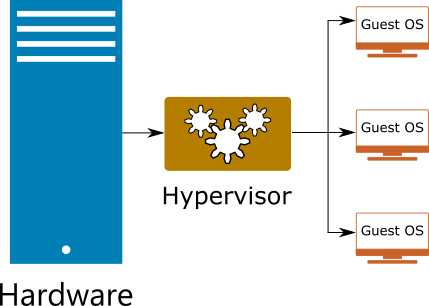
\includegraphics[scale=0.2]{hypervisor.png}
    \label{fig:univerise}
\end{figure}

\column{0.5\textwidth}
Niveau 2
\begin{itemize}
    \item VMware Workstation
    \item Oracle Virtual Box
\end{itemize}

\begin{figure}[htbp]
    \centering
    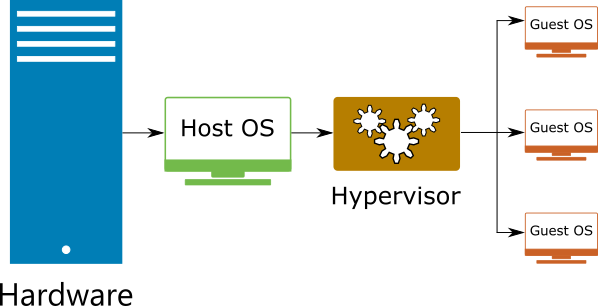
\includegraphics[scale=0.2]{hypervisor_2.png}
\end{figure}

% \column{0.33\textwidth}
% Containers
% \begin{itemize}
%     \item LXC
%     \item Docker / Kubernetes
% \end{itemize}

\end{columns}
\end{frame}
    
%====================================
%================5===================

\begin{frame}
\frametitle{Virtualisation de serveurs}

Technologies de virtualisation x86\_64: extensions des processeurs
\medbreak
\medbreak
Optimisation des ressources materielles (CPU, mémoire, disque)
\medbreak
\medbreak
Infrastructures en grappes (cluster) : haute disponibilité %(cluster)

\end{frame}

%====================================
%================5===================

\begin{frame}
\frametitle{Virtualisation de stockage}

Méthode de présentation de stockage aux hyperviseurs

\begin{itemize}
    \item SAN: Storage Area Network
    \item VSAN: Virtual SAN
    \item NAS: Network Access Storage
\end{itemize}

Choix: Infrastructure / Budget / Performance



% Dell / HP

% Virtualisation de stockage en SAN (100k euros): on a plus de disques physiques présentés
% mais des espaces de blocks. La repartition sur les disques est gérée automatiquement par la baie de
% stockage.
% Fibre: 16Gbit (voire 40Gbit)

% VSAN: aggrège l'ensemble des stockages des hyperviseurs dans un espace de stockage commun à l'infra virtuelle
% Comporte de la haute dispo (si un hyperviseur tombe, données encore accessibles) + du cache
% Réseau 10Gbit (voire 40Gbit)

% Baies NAS: entrée de gamme mais moins cheres, bien moins performant. Constructeur: Synology, protocole: NFS; SAMBA - SMB3
% Réseau classique 1Gbit

% Choix: infra / prix / performance


\end{frame}

%====================================
%================6===================

\begin{frame}
\frametitle{Virtualisation de réseau}

Virtualisation d'une ou plusieurs parties de la pile réseau

Elements physiques
\begin{itemize}
    \item Router, switch
    \item Pare-feu
\end{itemize}
Elements virtuels
\begin{itemize}
    \item Segmentation du réseau: VLAN, Overlay
    \item Optimisation: Load balancing
    \item Sécurisation: anti-spoofing, anti-ddos, VPN
\end{itemize}

Choix de la solution: 5 critères (Schéma de routage, garantie de bande passante, routage multi-chemin, partage de bande passante, coût)

\end{frame}

%====================================
%================7===================

\begin{frame}
\frametitle{Virtualisation de postes}

Mise en place de VDI (Virtual Desktop Infrastucture)

\begin{itemize}
    \item Centralisation des postes dans le datacenter
    \item Réduction des coûts: centralisation des configurations, sécurité des postes
\end{itemize}

Choix des outils
\begin{itemize}
    \item VMware Horizon
    \item Citrix XenDesktop
    \item Solutions sur mesure (RDP, SPICE)
\end{itemize}


\end{frame}

%====================================
%================8===================

\begin{frame}
\frametitle{Sauvegardes}
Element essentiel d'une infrastructure virtualisée
\medbreak
\medbreak
Mise en place de solutions integrées
\medbreak
\medbreak
Snapshots prises régulièrement

\end{frame}

%====================================
%================9===================

\begin{frame}
\frametitle{Résultats}

Simplification et optimisation des ressources
\medbreak
\medbreak
Industrialisation des centres de données
\medbreak
\medbreak
Réduction des coûts d'exploitation

\end{frame}

% Conlusion:
% Virtualisation de serveur: acquis
% Virtualisation de stockage : très souvent
% Virtualisation de réseaux: début d'industrialisation
% Virtualisation des postes de travail: dépend des structures

%====================================
%================11===================

\begin{frame}
\frametitle{Biliographie}
\begin{itemize}
    \fontsize{6pt}{7.2}\selectfont

    \item R. Buyya, R. N. Calheiros, J. Son, A. V. Dastjerdi and Y. Yoon, "Software-Defined Cloud Computing: Architectural elements and open challenges," 2014 International Conference on Advances in Computing, Communications and Informatics (ICACCI), New Delhi, 2014, pp. 1-12
    \item Bhore, Pratik. (2016). A Survey on Storage Virtualization and its Levels along with the Benefits and Limitations. INTERNATIONAL JOURNAL OF COMPUTER SCIENCES AND ENGINEERING. 4. 115-121.
    \item M. F. Bari et al., "Data Center Network Virtualization: A Survey," in IEEE Communications Surveys \& Tutorials, vol. 15, no. 2, pp. 909-928
    \item M. Alouane and H. El Bakkali, "Virtualization in Cloud Computing: Existing solutions and new approach," 2016 2nd International Conference on Cloud Computing Technologies and Applications (CloudTech), Marrakech, 2016, pp. 116-123
    \item Chrobak, Pawel. (2014). Implementation of Virtual Desktop Infrastructure in academic laboratories. 1139-1146.
    \item Nagesh, O \& Kumar, Tapas \& Venkateswararao, V.. (2017). A Survey on Security Aspects of Server Virtualization in Cloud Computing. International Journal of Electrical and Computer Engineering. 7. 1326-1336.
\end{itemize}

\end{frame}

\end{document}


%% Biblio:
% www.buyya.com/papers/SDCC-Keynote2014.pdf
% https://www.researchgate.net/publication/305933028_A_Survey_on_Storage_Virtualization_and_its_Levels_along_with_the_Benefits_and_Limitations
% https://scihub.wikicn.top/https://doi.org/10.1109/SURV.2012.090512.00043
% https://scihub.wikicn.top/https://doi.org/10.1109/CloudTech.2016.7847687
% https://scihub.wikicn.top/http://doi.org/10.15439/2014F213
% https://www.researchgate.net/publication/318271881_A_Survey_on_Security_Aspects_of_Server_Virtualization_in_Cloud_Computing